\documentclass{article}
\usepackage[utf8]{inputenc}
\usepackage{graphicx}
\usepackage{amsmath}
\usepackage{amsfonts}
\usepackage{amsbsy}
\usepackage{mathrsfs}
\usepackage{appendix}
\usepackage{amsthm}
\usepackage{bbold}
\usepackage{epstopdf}
\usepackage{stmaryrd}
\usepackage[]{algorithm2e}
\usepackage{multirow}
\usepackage{xcolor}
\newcommand{\red}[1]{\textcolor{red}{#1}}
\title{Project report for NPM3D : \\PCA based 3D point cloud classification}
\author{Leman FENG\\ Email: flm8620@gmail.com\\Website: lemanfeng.com}

\begin{document}
\maketitle
\section{Introduction}
After the mini-challenge of 3d point cloud classification in course, I decided to explore more on the subject of PCA based 3D points cloud classification. I read two articles \cite{weinmann2015} \cite{hackel2016fast} which present the state-of-art methods using PCA on neighborhoods. I will first summarize the two articles, then give some critical points of view, followed with a reproduction of method \cite{hackel2016fast} on a new dataset. At last I will give some new ideas on this subject together with test on a dataset.

\section{Article Summary}
The first article \cite{weinmann2015} provide a comprehensive comparison of different approaches in three aspects: neighborhood selection, feature design and classifier. And they proposed a better way of neighborhood selection. The second article \cite{hackel2016fast} focused on proposing a new pyramid grid sub-sampling and a new feature design. I will summarize the two article following the three aspects and their result on datasets.
\subsection{Neighborhood selection}
To tell the class of one point, the most natural way is to look at its neighborhoods. There are two ways of neighborhood selection : radius search and $k$ nearest neighbors. \cite{weinmann2015} and \cite{hackel2016fast} give different approaches. 

The first article \cite{weinmann2015} wants to find a optimal sizing of neighborhoods in the sense that the selection gives the most information on PCA features. They use $k$-NN from $k=10$ to $100$ and find the best $k$ maximizing the eigen-entropy:
\begin{equation}
E_\lambda = -\sum_{i=1}^{3} e_i \log e_i
\end{equation}
where $e_i = \lambda_i/\sum_{j=1}^{3} \lambda_j$.

And they use the best $k$ as the best and only scale to generate PCA features. They shown in tests that their eigen-entropy criterion gives better result in most of the time compared to different fixed $k$-NN and other optimal size criteria.

The second article \cite{hackel2016fast} use multi-scale neighborhood with $k$-NN. They firstly subsample the point cloud by voxel grids with grid sizing varying from 0.025m to 6.4m, each time multiplied by a factor of 2, totally 9 scales. They hope the sub-sampling can skip dense points for acquiring invariance to density. And this sub-sampling can help reduce the neighborhood querying time.

For each scale, they then fix $k=10$ for $k$-NN and do PCA on these 10 points.
\subsection{Feature design}
Most of features selected in two articles are based on eigenvalue and eigenvector of the PCA on neighborhoods. 
The second article \cite{hackel2016fast} uses 16 features. Shown in Table \ref{table:1}.
\begin{table}[h!]
	\centering
	\begin{tabular}{|c | c | c |} 
		\hline
		\multirow{9}{*}{Covariance}
		& Sum & $\sum_{i=1}^{3}\lambda_i$ \\ 
		& Omnivariance & $(\lambda_1 \lambda_2 \lambda_3)^{\frac{1}{3}}$ \\ 
		& Eigenentropy & $-\sum_{i=1}^{3}\lambda_i \log \lambda_i$ \\ 
		& Anisotropy & $(\lambda_1-\lambda_3)/\lambda_1$ \\ 
		& Planarity & $(\lambda_2-\lambda_3)/\lambda_1$ \\ 
		& Linearity & $(\lambda_1-\lambda_2)/\lambda_1$ \\ 
		& Surface Variation & $\lambda_3/(\lambda_1+\lambda_2+\lambda_3)$ \\ 
		& Sphericity & $\lambda_3/\lambda_1$ \\ 
		& Verticality & $1-|\langle [0,0,1], \mathbf{e}_1\rangle|$ \\ 
		\hline
		\multirow{4}{*}{Moment}
		& 1\textsuperscript{st} order, 1\textsuperscript{st} axis  & $\sum_{i\in \mathcal{N}}\langle \mathbf{p}_i-\mathbf{p}, \mathbf{e}_1\rangle$ \\ 
		& 1\textsuperscript{st} order, 2\textsuperscript{nd} axis & $\sum_{i\in \mathcal{N}}\langle \mathbf{p}_i-\mathbf{p}, \mathbf{e}_2\rangle$ \\ 
		& 2\textsuperscript{nd} order, 1\textsuperscript{st} axis & $\sum_{i\in \mathcal{N}}\langle \mathbf{p}_i-\mathbf{p}, \mathbf{e}_1\rangle^2$ \\ 
		& 2\textsuperscript{nd} order, 2\textsuperscript{nd} axis & $\sum_{i\in \mathcal{N}}\langle \mathbf{p}_i-\mathbf{p}, \mathbf{e}_2\rangle^2$ \\ 
		\hline
		\multirow{4}{*}{Height}
		& Vertical range & $z_{\text{max}}-z_{\text{min}}$ \\ 
		& Height below & $z-z_{\text{min}}$ \\ 
		& Height above & $z_{\text{max}}-z$ \\ 
		\hline
	\end{tabular}
	\caption{16 features used in \cite{hackel2016fast}}
	\label{table:1}
\end{table}
Most features of ``covariance'' in Table \ref{table:1} are also tested in \cite{weinmann2015}. The four ``Moment'' features take the neighborhood's offset into account, which can increase precision for boundary points, according to \cite{hackel2016fast}.

The ``Height'' features are measured in a cylindrical neighborhood. And there is a $5\%$ drop in precision if they are not used, according to \cite{hackel2016fast}.

In the first article \cite{weinmann2015}, they also tested other non-PCA feature such as 2D features. And from the test in \cite{weinmann2015}, we can conclude basically more features you use, better precision you get. 
\subsection{Classification}
\cite{weinmann2015} shown that Random Forest has good performance in most of time. And for this reason, \cite{hackel2016fast} only test on Random Forest.

\subsection{Dataset \& Result}
The first article \cite{weinmann2015} used the \textit{Oakland 3D Point Cloud Dataset} and \textit{Paris-rue-Madame database}. And the second article used \textit{Paris-rue-Madame database} and \textit{Paris-Rue-Cassette database}.

\textit{Oakland 3D Point Cloud Dataset} is already separated in training, validation and test sets. While \textit{Paris-rue-Madame database} is not separated. For \textit{Paris-rue-Madame database} and \textit{Paris-Rue-Cassette database}, both articles conduct a class re-balancing and randomly select 1000 points per class as training set, and rest points for test set.

\section{Criticism}
\subsection{Neighborhood selection}\label{sec:nb}
The selection of neighborhood is always the same story, either by querying points in a ball(or $k$-NN) with optimal radius(or $k$), or multiple balls with fixed sizes stacked together.

I think if the scale of dataset is known, such as 1 unit = 1 meter (and for most cases, it is. Because most data are laser scanned), then fixed radius querying makes sense because each type of object always gives the most useful information on a specific scale, for example, cars are always several meters long, pedestrians are always 1-2 meters tall.

But I don't think the multi-scaled concentric balls is the optimal solution. Most 3D features are related to PCA. The problem of PCA is that it basically represents the best ellipsoid that approximates your neighborhoods. If the ball is large, it covers more points, but an approximated ellipsoid is too abstract for a large coverage. And if the ball is small, PCA is a good local descriptor for shapes like line, plane, etc. But a small ball cover few points. There is always a dilemma of scale and detail.

\subsection{Feature design \& Classification}
\subsubsection{Unclear definition}
In both article, they all said three eigenvalues should be normalized such that the sum is one. But then they introduced the eigensum feature $\Sigma_\lambda = \sum_{i=1}^{3} \lambda_3$ AFTER this normalization. But they also use the eigenentropy term as a feature with the same symbol of eigenvalue as eigensum. For my reproduction, I will take eigensum as the sum of raw eigenvalues and use the normalized eigenvalues for all rest features.

\subsubsection{Hand craft features}\label{sec:features}
It seems that the key of point cloud classification is the design of your feature. More delicately crafted features you get, better the result is. I don't think this is the right way to go. PCA on neighborhood only provide 6 degrees of freedom, 3 for eigenvalues, 3 for a orthogonal basis of three eigenvectors. \cite{hackel2016fast} used 9 PCA features, and 8 of them only depend on eigenvalues. Which means you need to map your 3 eigenvalues into a higher dimension space that can make your random forest happy. 

I think the problem is, random forest is sensible to your feature design. The only thing a decision tree can do is to divide recursively your data by one feature value each time. So it's hard for a decision tree, given raw eigenvalues, to decide according to some function of them, for example, the linearity in function of eigenvalues: $L(\lambda_1,\lambda_2,\lambda_3) = (\lambda_1-\lambda_2)/\lambda_1$.

Why not let the machine to learn the best descriptors, instead of those hand craft features? Just like the Convolutional Neural Networks that can learn basic descriptors on images in the first several layers.

Besides, I don't think using the height information of points is a good idea. This features prevents translation invariance. Yes, most dataset has flat ground, and most pedestrians and cars are always on the ground. What about a car on a bridge going above a building ? The correct logic should bases on the space relationship. For example, a car-like object on a flat surface should be a car. A vertical cylinder under fuzzy points should be a tree, not a lamp-post. So for the following test, I deleted height features, which will decrease the precision by $5\%$ \cite{hackel2016fast}, according to their test.

\subsection{Dataset \& Result}
I don't agree with the way by which both article generate data from the \textit{Paris-rue-Madame database} and \textit{Paris-Rue-Cassette database}. They pick 1000 points per class randomly from point cloud, and the rest points become the test data. You cannot create training data and test data from the same point cloud. Simply because many testing points will have some neighbors belonging to 1000 points for training, and features for neighboring points are very similar. I'm afraid the $97\%$ overall precision in \cite{hackel2016fast} is just a over-fitting on training set.

\section{New ideas}
\subsection{Neighborhood selection}
\subsubsection{Voxel grid subsampling}
I will use the multi-scale voxel grid subsampling as \cite{hackel2016fast}, for the efficiency of querying and for a uniform density on point clouds. But I will use radius querying instead of $k$-NN because I think a fixed radius can well capture the geometry at specific scale. 

I adapt the size of voxel grid to the radius of query. In practice, I take voxel grid size as $\frac{1}{4}$ of the radius.

\subsubsection{Neighborhood's Neighborhood}
To solve the dilemma mentioned in Section \ref{sec:nb}, I propose a new method called Neighborhood's Neighborhood. Instead of querying only by one ball centered at the point $\mathbf{p}$ to classify, I query 6 more balls surrounding the center ball : 

Let $\{\mathbf{e}_i\}_{i}$ be the three eigenvectors from result of PCA of the center ball, corresponding to three eigenvalues: $\{\lambda_i\}_{i}$ and $\lambda_1 \geq \lambda_2 \geq \lambda_3$. Let $R$ be the radius of the center ball. Then the 6 surrounding balls are centered at:
\begin{equation}
\mathbf{p}\pm \mu R \mathbf{e}_i,\quad i=1,2,3
\end{equation}
and they have the same radius as the center ball. In practice, I take $\mu=1.5$

I use in total 4 scales, from 0.1m to 2.7m with a multiplication factor of 3 instead of 2 because with surrounding balls, each scale covers more points.

\subsection{Feature design}
I don't want to design any complicated features manually. I want to provide directly raw features from PCA, and then feed it into a convolutional neural network.

Let's define $\{\lambda_i\}_{i}$ and $\lambda_1 \geq \lambda_2 \geq \lambda_3$ as the raw eigenvalues from PCA. And $\Sigma_\lambda = \sum_{j=1}^{3}\lambda_j$ And $l_i = \lambda_i / \Sigma_\lambda$ as normalized eigenvalues.

Recall that $\Sigma_\lambda$ are actually the sum of squared distance to centroid of all points. So if we want to include $\Sigma_\lambda$ as a raw feature, it's better to normalize it as ${\Sigma_\lambda}/{R^2}$

For eigenvectors, the only feature I want to take is the verticality : 

$$\frac{2\arcsin(|\langle [0,0,1], \mathbf{e}_1\rangle|)}{\pi} \in [0, 1]$$

At last, for all balls at the same scale, I add the "density ratio to center ball" which is the ratio between number of neighbors $N$ in ball compared to which in center ball $N_c$. For consistency, this value is set to 1.0 for center ball.

For summary, the raw features I take are : 
\begin{table}[h!]
	\centering
	\begin{tabular}{| c | c |} 
		\hline
		Density ratio to center ball & $N / N_c$\\
		\hline
		Normalized eigensum & ${\Sigma_\lambda}/{R^2}$ \\ 
		\hline
		\multirow{3}{*}{Normalized Eigenvalues}
		& $\lambda_1/\Sigma_\lambda$ \\
		& $\lambda_2/\Sigma_\lambda$ \\
		& $\lambda_3/\Sigma_\lambda$ \\
		\hline
		Verticality & $2\arcsin(|\langle [0,0,1], \mathbf{e}_1\rangle|) / \pi$\\
		\hline
	\end{tabular}
	\caption{features}
	\label{table:2}
\end{table}

There are 4 scales, 7 balls for each scale and 6 features for each ball. In total 168 features.


\subsection{Classification}
I test three different classifiers, the first one is random forest, the second one is Multi-Layer Percepton. Then I propose a convolutional neural network as following:

\begin{figure}[h]
	\centering
	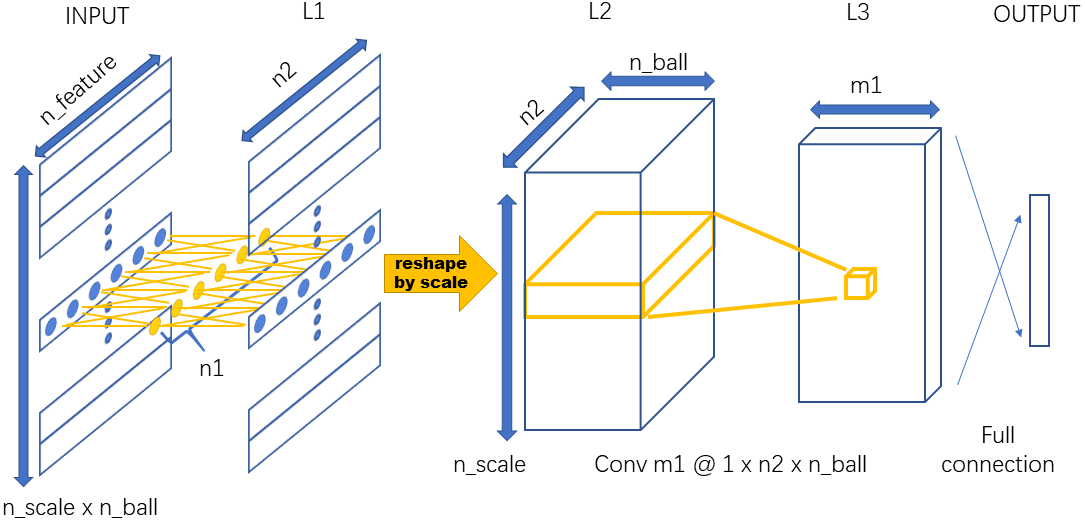
\includegraphics[width=12cm]{cnn.png}
	\caption{Convolutional Neural Network}
	\label{fig:cnn}
\end{figure}

Note ``n\_scale'', ``n\_ball'' and ``n\_feature'' as the number of scale, number of balls for each scale and number of features for each ball. 

The input is a matrix with size (n\_scale*n\_ball, n\_feature). Each row is a feature vector for one ball. 

Then I apply a small MLP on all feature vectors to map the feature space to another space with dimension ``n3'' (Layer ``L1''). The weight of this MLP is shared among all features, which is different from traditional MLP. This convolutional-like small MLP let the network to learn the best function of features.

Layer ``L1'' is reshaped to ``L2'', a 3D tensor of size (n\_scale, n\_ball, n3). Each floor of ``L2'' represent features in all balls at same scale.

A convolution is apply to ``L2'' with kernel size (1, n3, n\_ball), and in total m1 kernels. The idea of convolution is that a useful MLP for one scale are probably useful for other scales. For each scale, this MLP maps all features into a vector of length m3.

Finally, ``L3'' is full connected to a flatten layer ``L4'', which is then full connected to the output.

In practice, the parameters of layer structures is shown in Table \ref{table:3}

\begin{table}[h!]
	\centering
	\begin{tabular}{|c|c|c|c|c|} 
		\hline
		n1 & n2 & n3 & m1 & L4\\
		\hline
		? & ? & ? & ? & ?\\
		\hline
	\end{tabular}
	\caption{Parameters of network structure}
	\label{table:3}
\end{table}


\subsection{Dataset}
\begin{figure}[h]
	\centering
	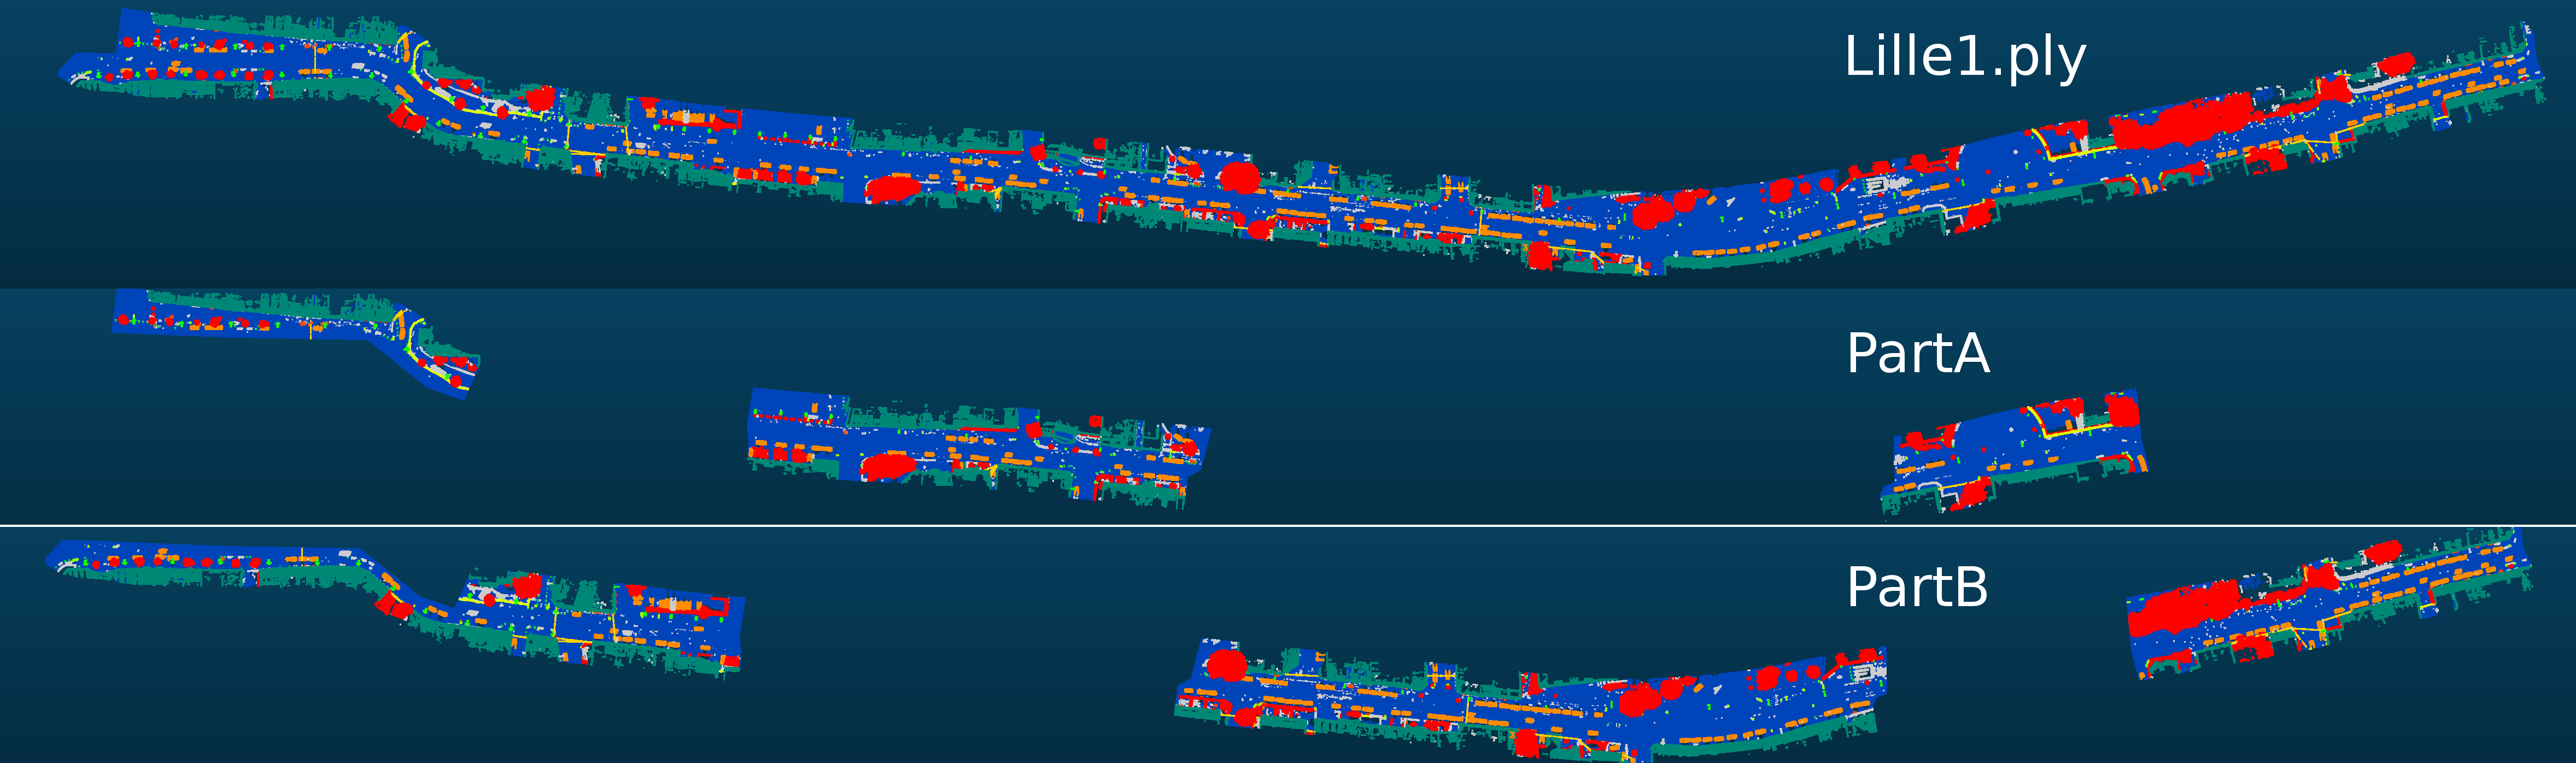
\includegraphics[width=12cm]{Lille1_cut.png}
	\caption{Data separation for Lille1.ply}
	\label{fig:lill1}
\end{figure}

I choose the Paris-Lill1-3D dataset \cite{2017arXiv171200032R}. The dataset comes with 3 files: Lille1.ply, Lille2.ply and Paris.ply. I only use the first file.

To avoid data overlapping which causes false high precision in \cite{hackel2016fast} and \cite{weinmann2015}, I demand that training data and test data shall not come from the same part of the point cloud. To assure the data separation, I cut the point cloud manually into two parts A and B as shown in Fig \ref{fig:lill1}.


I didn't cut it directly into 2 parts, but pick specific regions. Because I need assure that we have similar structures in both part. For example, the left most street is cut in half through the road because the shape of boder tree there doesn't appear in other parts. So I separate the left/right hand sides of road into two part.

The dataset come with very detailed class labels on each point using the \textit{class tree} of iQmulus/Terramobilita benchmark. I did a remapping of class labels into 11 simplified classes, and ignore some classes with too few samples. The remapping is shown in Table \ref{table:class}.

\begin{table}[h!]
	\centering
	\begin{tabular}{|c|c|c|c|} 
		\hline
		My class & Description & Original class & Description\\
		\hline
		\multirow{3}{*}{0} & \multirow{3}{*}{Unknown} &
		(All other classes) & (All other classes)\\
		& & 000000000  & unclassified \\
		& & 100000000  & other \\
		\hline
		\multirow{4}{*}{1} & \multirow{4}{*}{Ground} &
		202020000 & road \\
		& & 202030000 & sidewalk \\
		& & 202050000 & island \\
		& & 202060000 & vegetal ground\\
		\hline
		2 & Building & 203000000 & Building \\
		\hline
		3 & Bollard & 302020300 & Bollard \\
		\hline
		4 & Floor lamp & 302020400 & Floor lamp \\
		\hline
		5 & Traffic light & 302020500 & Traffic light \\
		\hline
		\multirow{2}{*}{6} & \multirow{2}{*}{Sign} &
		302020600  & Traffic sign \\
		& & 302020700  & Signboard \\
		\hline
		7 & Roasting & 302030300 & Roasting \\
		\hline
		8 & Wire & 302030600 & Wire \\
		\hline
		9 & 4+ Wheels & 303040*** & 4+ Wheels \\
		\hline
		10 & Trash can & 303050500 & Trash can \\
		\hline
		\multirow{3}{*}{11} & \multirow{3}{*}{Natural} &
		    304000000  & Natural\\
		& & 304020000  & Tree \\
		& & 304040000  & Potted plant \\
		\hline
	\end{tabular}
	\caption{Remapping of class}
	\label{table:class}
\end{table}

\subsection{Result}
I use data part A for training and part B for testing. In part A, I pick as most 10000 samples per class for traning. And as most 20000 per class in part B for testing. Number of training and testing samples per class is shown in Table \ref{table:samples}.

\begin{table}[h!]
	\centering
	\makebox[\textwidth][c]{
	\begin{tabular}{|c|c|c|c|c|c|c|c|c|c|c|c|} 
		\hline
		& ground & building & bollard & floor lamp & traffic light & sign & roasting & wire & 4+ wheels & trash can & natural\\
		\hline
		Training & 10000 & 10000 & 10000 & 10000 & 10000 & 10000 & 10000 &  1973 & 10000 & 10000 & 10000 \\
		\hline
		Testing  & 20000 & 20000 & 17256 & 20000 &  7987 & 20000 & 20000 & 12211 & 20000 & 20000 & 20000 \\
		\hline
	\end{tabular}
	}
	\caption{Remapping of class}
	\label{table:samples}
\end{table}

I tested the method in Section \cite{hackel2016fast}, but I removed all height features for reason stated in \ref{sec:features}. So there are balls in 9 scales from 0.025m to 6.25m, and 13 features for each scale, in total 117 features. The result is shown in Table \ref{table:timo}.

For MLP, I use \red{?} layers with width of \red{?}. There are \red{?} parameters in my MLP and \red{?} parameters for my CNN.

\begin{table}[h!]
	\centering
	\makebox[\textwidth][c]{
		\begin{tabular}{|c|c c c|c c c|c c c|} 
			\hline
			 & \multicolumn{3}{|c|}{Random forest} & \multicolumn{3}{|c|}{MLP} & \multicolumn{3}{|c|}{Convolutional}\\
			\hline
			 & precision & recall & f1-score & precision & recall & f1-score & precision & recall & f1-score\\
			\hline
ground			& 96.1 & 96.3 & 96.2 & 93.4 & 95.2 & 94.3 & 94.2 & 95.1 & 94.6 \\
building		& 53.2 & 89.9 & 66.8 & 67.3 & 83.0 & 74.3 & 67.7 & 84.2 & 75.1 \\
bollard			& 93.5 & 50.2 & 65.3 & 84.5 & 57.2 & 68.2 & 87.9 & 77.2 & 82.2 \\
floor lamp		& 46.0 & 77.7 & 57.8 & 46.6 & 71.2 & 56.4 & 65.6 & 71.1 & 68.2 \\
traffic light	& 71.4 & 03.7 & 07.0 & 62.0 & 23.5 & 34.1 & 78.3 & 59.5 & 67.6 \\
sign			& 32.9 & 12.6 & 18.2 & 23.9 & 24.3 & 24.1 & 32.0 & 38.4 & 34.9 \\
roasting		& 39.5 & 56.5 & 46.5 & 47.5 & 68.2 & 56.0 & 53.3 & 50.8 & 52.1 \\
wire			& 99.3 & 38.1 & 55.0 & 87.6 & 43.7 & 58.3 & 88.1 & 62.0 & 72.8 \\
4+ wheels		& 69.0 & 88.8 & 77.7 & 75.1 & 73.9 & 74.5 & 78.3 & 78.4 & 78.3 \\
trash can		& 45.9 & 26.5 & 33.6 & 47.3 & 45.1 & 46.2 & 54.9 & 53.7 & 54.3 \\
natural			& 41.3 & 81.5 & 54.8 & 55.5 & 70.4 & 62.0 & 59.1 & 70.1 & 64.1 \\
                                                                        
avg / total		& 62.6 & 56.5 & 52.6 & 62.8 & 59.6 & 58.9 & 69.0 & 67.3 & 67.7 \\
			\hline
			\end{tabular}
	}
	\caption{Test Result with method \cite{hackel2016fast}}
	\label{table:timo}
\end{table}

\begin{table}[h!]
	\centering
	\makebox[\textwidth][c]{
		\begin{tabular}{|c|c c c|c c c|c c c|} 
			\hline
			& \multicolumn{3}{|c|}{Random forest} & \multicolumn{3}{|c|}{MLP} & \multicolumn{3}{|c|}{Convolutional}\\
			\hline
			& precision & recall & f1-score & precision & recall & f1-score & precision & recall & f1-score\\
			\hline
			ground			& ??? & ???? & 96.2 & 93.4 & 95.2 & 94.3 & 94.2 & 95.1 & 94.6 \\
			building		& ??? & ???? & 66.8 & 67.3 & 83.0 & 74.3 & 67.7 & 84.2 & 75.1 \\
			bollard			& ??? & ???? & 65.3 & 84.5 & 57.2 & 68.2 & 87.9 & 77.2 & 82.2 \\
			floor lamp		& ??? & ???? & 57.8 & 46.6 & 71.2 & 56.4 & 65.6 & 71.1 & 68.2 \\
			traffic light	& ??? & ???? & 07.0 & 62.0 & 23.5 & 34.1 & 78.3 & 59.5 & 67.6 \\
			sign			& ??? & ???? & 18.2 & 23.9 & 24.3 & 24.1 & 32.0 & 38.4 & 34.9 \\
			roasting		& ??? & ???? & 46.5 & 47.5 & 68.2 & 56.0 & 53.3 & 50.8 & 52.1 \\
			wire			& ??? & ???? & 55.0 & 87.6 & 43.7 & 58.3 & 88.1 & 62.0 & 72.8 \\
			4+ wheels		& ??? & ???? & 77.7 & 75.1 & 73.9 & 74.5 & 78.3 & 78.4 & 78.3 \\
			trash can		& ??? & ???? & 33.6 & 47.3 & 45.1 & 46.2 & 54.9 & 53.7 & 54.3 \\
			natural			& ??? & ???? & 54.8 & 55.5 & 70.4 & 62.0 & 59.1 & 70.1 & 64.1 \\
			
			avg / total		& 62.6 & 56.5 & 52.6 & 62.8 & 59.6 & 58.9 & 69.0 & 67.3 & 67.7 \\
			\hline
		\end{tabular}
	}
	\caption{Test Result with my method}
	\label{table:leman}
\end{table}
\bibliographystyle{unsrt}
\bibliography{sample}
\end{document}



































